An appropriate combination of swarm intelligence \cite{MOEA07} and a generalized allocation problem (GAP) strategy \cite{ferreira2007swarm} allows to generate an algorithm, based on token transmissions, that the agents perceives  in the environment or receives them from a central unity, and does the correct and optimized allocation among the agents. Its pseudo code is presented in Algorithm \ref{algo:swarm-gap} (from original in \cite{MAS07}). 

The work here proposed is based on three variations of swarm-GAP to solve an allocation problem among a team of agents, presented by Schwarzrock et al. in \cite{MAS07}. The task allocation is modeled as a generalized assignment problem (GAP) and the goal is to maximize the total capability of the agents using a probabilistic approach \cite{theraulaz1998response}.

\begin{algorithm}[!ht]
	\SetAlgoLined
	\DontPrintSemicolon
	\SetKwBlock{Loop}{loop}{end loop}
	\SetKwFor{ForAll}{for all}{do}{end for}
	\SetNlSty{text}{}{:}
	\SetNlSkip{0.3em}	
	
	\caption{Pseudo code of the Swarm-GAP (from Schwarzrock et al.) }
	\label{algo:swarm-gap}
	Receive Token\; \label{line:receivetoken}
	Compute available resources $r_i $ \; \label{line:compute_r}
	\ForAll{ available tasks }{ \label{line:forall}
		Compute capability $k_{ij}$\; \label{line:compute_k}
		Compute tendency $T_{\theta_{ij}(st)}$ \;  \label{line:compute_t}
		\If{ roulette() $< T_{\theta_{ij}(st)}$ and $r_i \geq c_j $}{ \label{line:ini_ifalgo1}
			Allocate task $j$ to agent $i$ \; \label{line:aloca_sgap}
			Decrease resource $r_i $\; \label{line:decrease_r} \label{line:fim_ifalgo1}
		}
	}
	Mark agent as visited in the token\; \label{line:marcavisitado}
	\If{there are still available tasks}{ \label{line:ifstillavatask}
		Send the token to a not yet visited agent\; \label{line:envia}
	}
\end{algorithm}


The purpose of this work is to present the results of the analysis about the reproducible research (RR) level of the original study. According to Madeyski and Kitchenham in \cite{exp02} the RR is referenced to the level how the experiment can be reproduced from the original data and information by others researchers. With a reproduction, the results obtained by the primary work can be validated and the information published completeness can be checked. Besides there is a significant difference between the concepts of RR and replication \cite{exp02} \cite{exp03}.

Elements of impact on experiment reproducibility level can be seen in Figure \ref{grafico:elements} adapted from González et al. in \cite{exp05}. Each of these elements represents an object that can be reused in a new research. The data source is the repository or object that has all data of experiment interest. Raw Dataset represents all data retrieved, normally using a software tool, from the data source. All data extracted from the Dataset represents a processed Dataset and, after an analysis, these information generates a result Dataset.

\begin{figure}[h]
	\begin{center}
		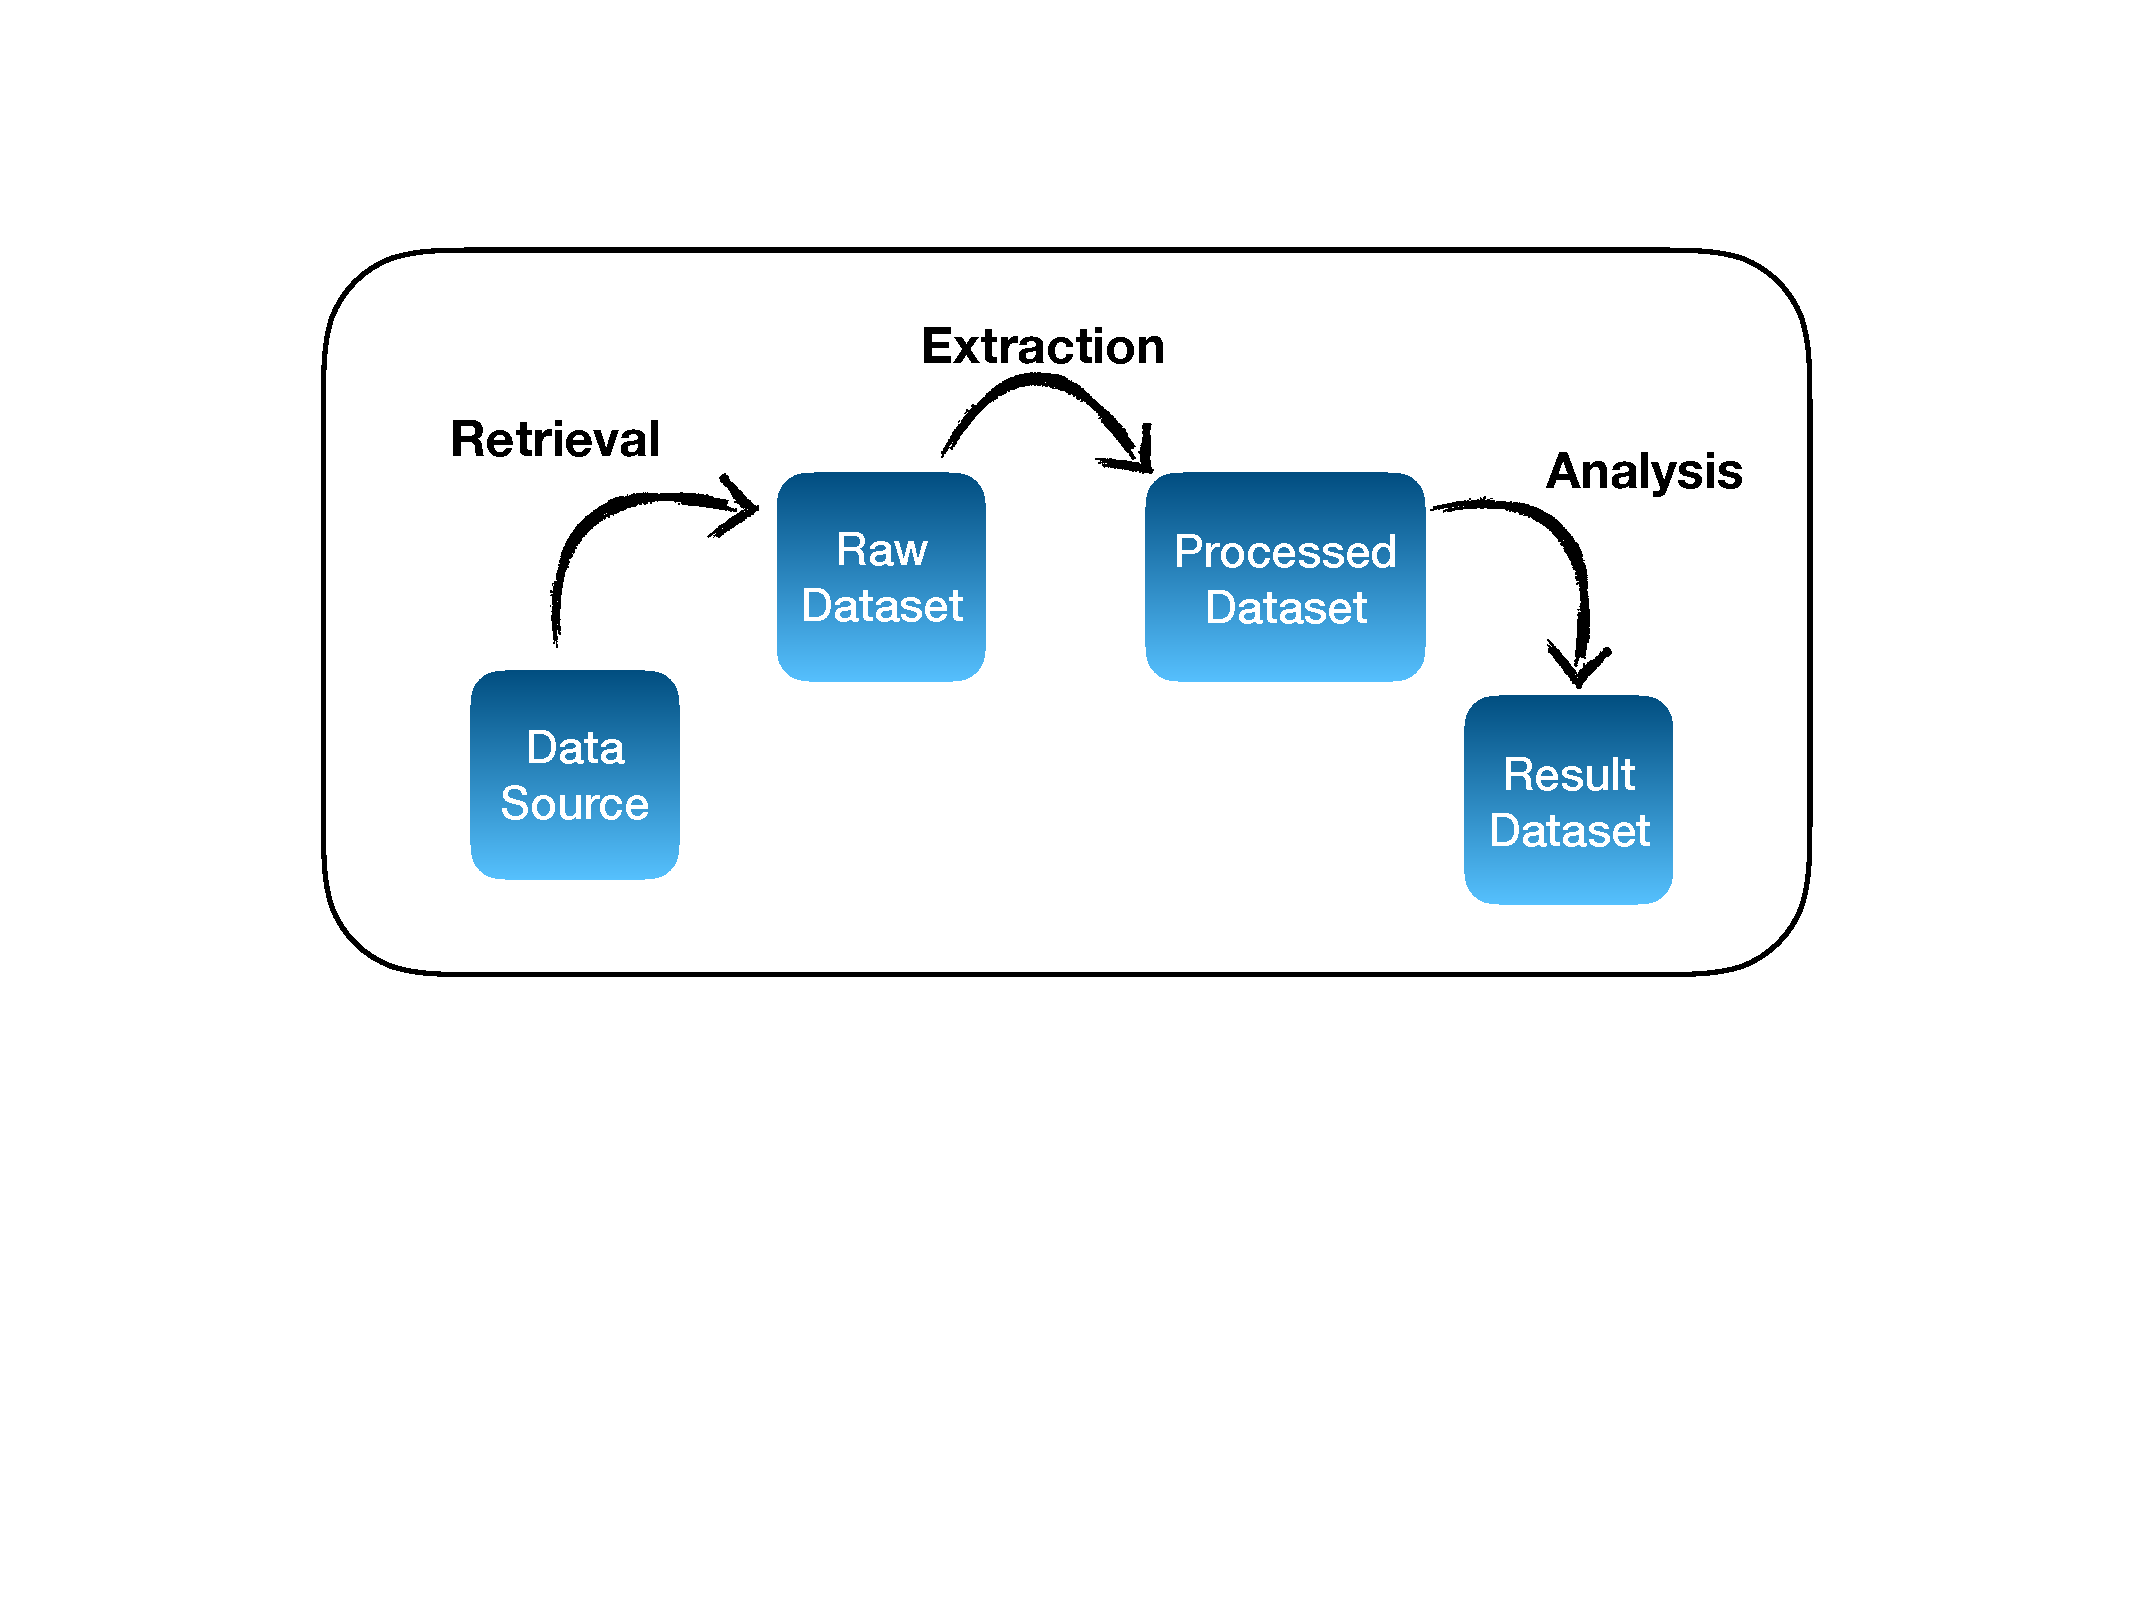
\includegraphics[scale=.35]{diagrama01.pdf}
		\caption{Elements of interest for reproducibility (Adapted from González et al.)}
		\label{grafico:elements}
	\end{center}
\end{figure}

This model was proposed to represent the data retrieving and processing in a empirical software engineer study \cite{exp05}. The main idea is to identify elements that can be reused during the experiment replication and to measure its reproducibility.

Replication in its all levels and types presented by González et al. in \cite{exp03} can creates different contexts from the original study or experiment. Variables, conditions and controls can be change to analyze the effects and impacts over the results. In empirical software engineer studies is common to apply replication in experiments to analyze the system behaviour under some conditions changes.

A specific case of replication called exact replication \cite{exp04} follows all procedures of an experiment as closely as possible to determine how the results obtained will be equals to the original experiment. In this case, the concepts reproduction and replication become the synonyms. The opposite situation occurs with the conceptual replication, where a different experimental procedures are used to prove hypotheses and to answer the research questions. 














